\subsection{Bayesian Optimisation}
The algorithm as supplied uses a greedy approach that does not work at all to find the global optimum in the case of the function we are given here. The function approximation $f^*$ will almost always have its minimum in the leftmost point, at $-1$, because this point has the lowest value $f(-1)$, of the dataset $\mathcal{D}$. However, this is not just a problem specific to this function. The algorithm will almost always reach this case after just a few iterations, where a point in the dataset becomes the minimum of $f^*$. When this becomes the case, the algorithm reaches a degenerate case where it only adds new data points on top of existing points, and as such we get next to no new information about the true function $f$. This means the approximation will not get better, and as such we cannot find a better minimum. For the algorithm to find the global minimum in its current state, we would need to have significantly more datapoints, with some of them already close to the minimum. The results of running the algorithm for 10 iterations can be seen in Figure \ref{fig:iter_naive}. We see that there is essentially no change between the different iterations, apart from the variance estimates. This is because all iterations in between are virtually identical, due to it finding a local optimum right away, and never doing any kind of exploration. It is important to note that the variance estimates in some cases are so significantly underestimated, that they are not visible in the plots.

\begin{figure}[h]
\centering
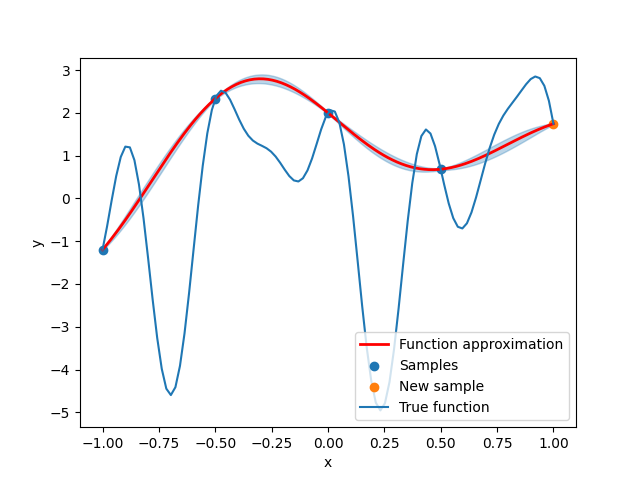
\includegraphics[width=0.3\linewidth]{images/bayesian_optimization_0.png}
%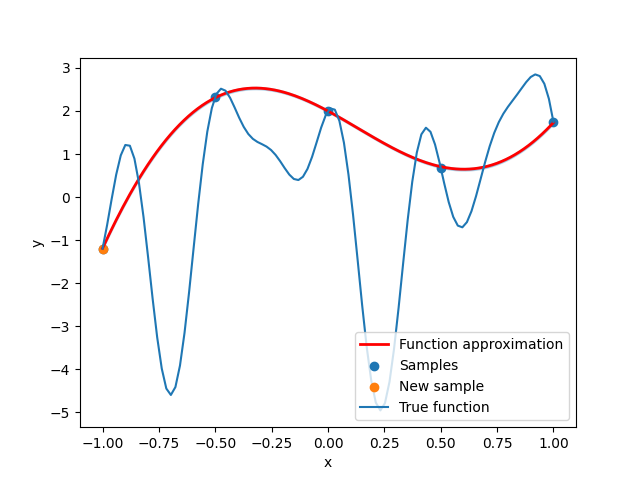
\includegraphics[width=0.3\linewidth]{images/bayesian_optimization_1.png}
%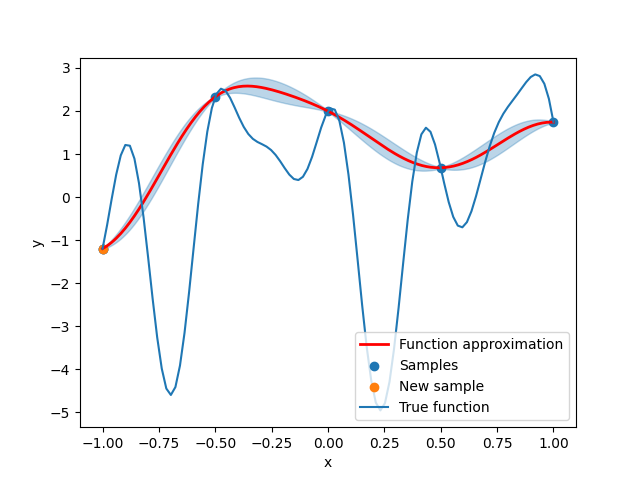
\includegraphics[width=0.3\linewidth]{images/bayesian_optimization_2.png}
%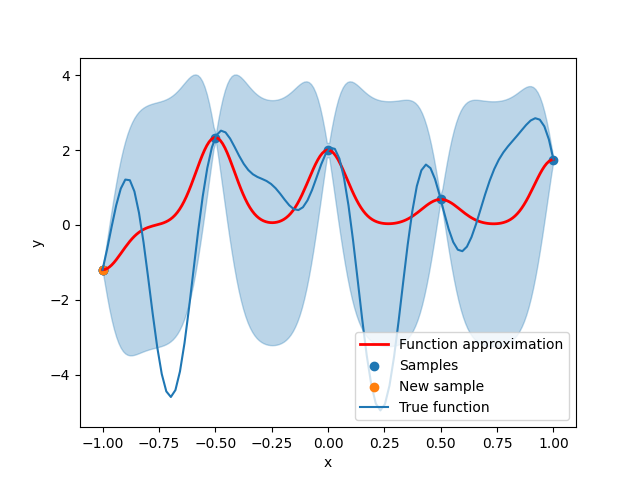
\includegraphics[width=0.3\linewidth]{images/bayesian_optimization_3.png}
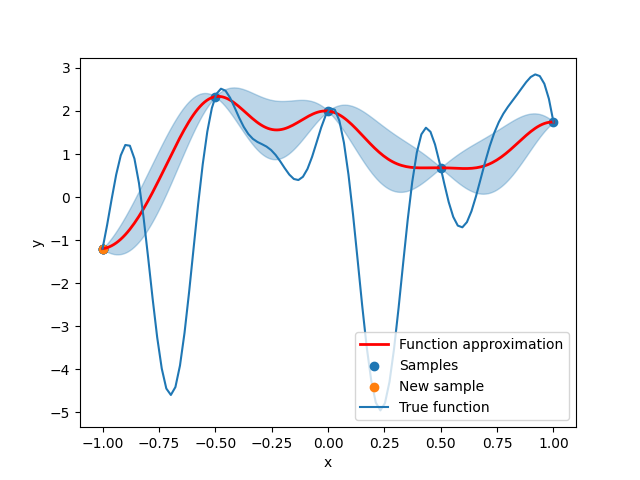
\includegraphics[width=0.3\linewidth]{images/bayesian_optimization_4.png}
%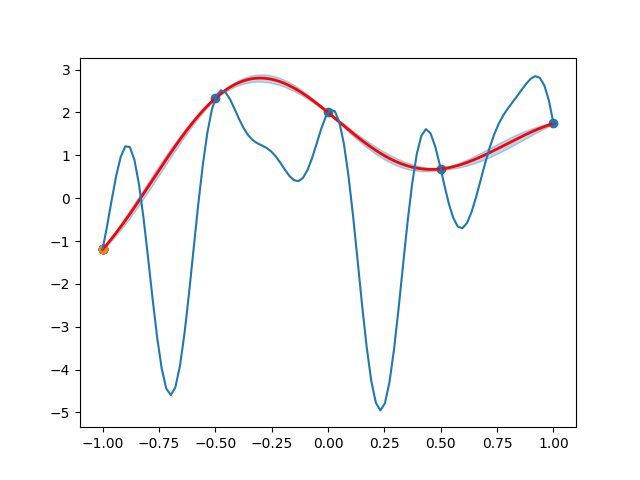
\includegraphics[width=0.3\linewidth]{images/bayesian_optimization_5.png}
%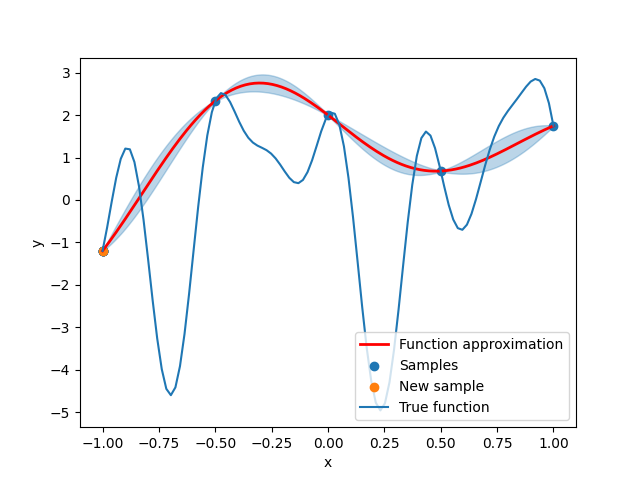
\includegraphics[width=0.3\linewidth]{images/bayesian_optimization_6.png}
%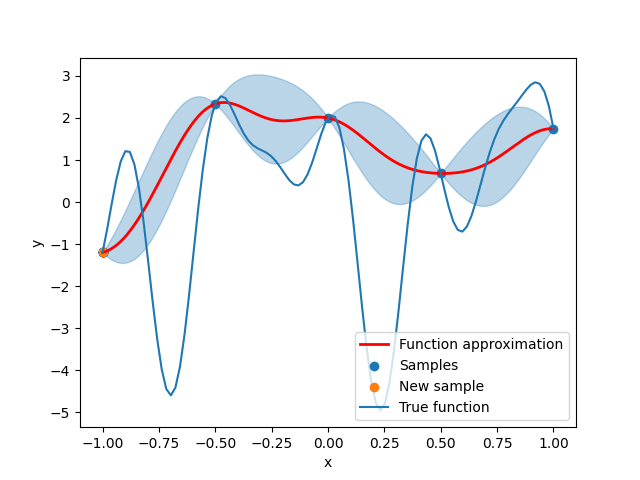
\includegraphics[width=0.3\linewidth]{images/bayesian_optimization_7.png}
%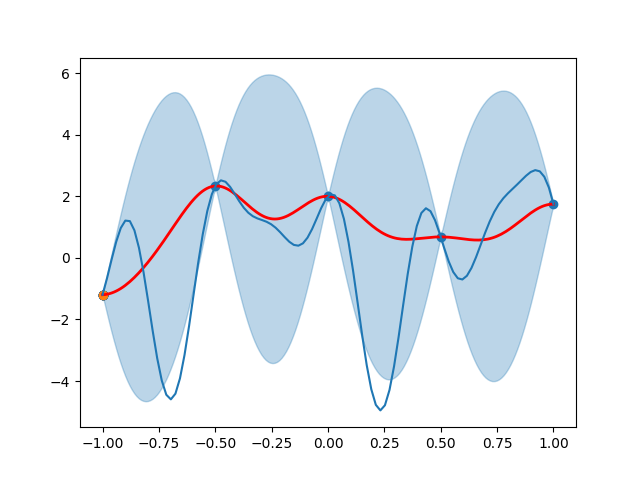
\includegraphics[width=0.3\linewidth]{images/bayesian_optimization_8.png}
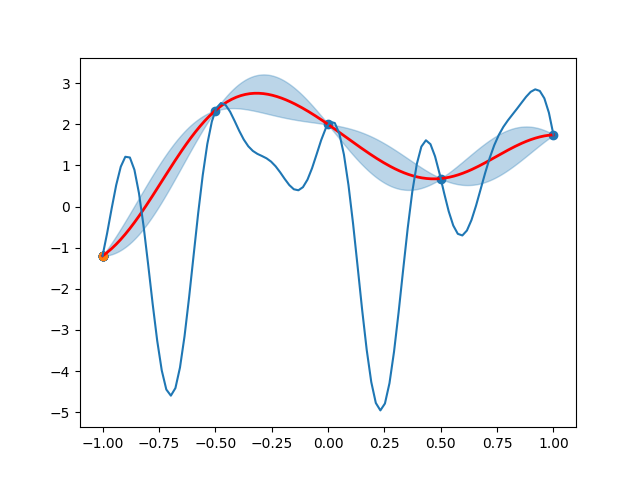
\includegraphics[width=0.3\linewidth]{images/bayesian_optimization_9.png}
\setlength{\belowcaptionskip}{-10pt}
\caption{Function approximation after 0, 5 and 10 iterations, adding each new data point according to the algorithm given. Notice that all new points are close enough the starting points to be indistinguishable.}
\label{fig:iter_naive}
\end{figure}

To fix these shortcomings, we first thought of going in the other direction from the supplied algorithm, and making ours such that it explores the function space better. The idea was that with sufficient exploration, we would hopefully find the global minimum, instead of just a local one. We did this by sampling $p = \texttt{argmax} \left( v(x^*), x^* \in X^*\right)$. This formulation would essentially only perform exploration, and as such find a much better function approximation very quickly. However, we realised that this formulation would often find the general area of the global minimum, but would never explore it without significantly more iterations. To fix this we ended up swapping between the two methods, every second step. The result is a very simple and elegant formulation that both explores the function space to try and find the global optimum, and explores the current best optimum, to improve that. This formulation also allows for another hyperparameter, namely tuning how often it tries to explore its current optimum, and how often it tries to explore the wider function space. More formally, we choose $p$ in the following way:

\begin{align}
  p &=
  \begin{cases}
    \texttt{argmax} ( v(x^*), x^* \in X^*), & \text{if } $x \% 2 = 0$\\
    \texttt{argmin}_i (f_i^*), & \text{if } $x \% 2 = 1$
  \end{cases}
\end{align}

Our results with this formulation can be seen in Figure \ref{fig:iter_new}. The resulting plots very obviously approximate the real function much better than the original algorithm, which leads to it exploring other minima than just the one found in the first iteration. We even see that in iteration 5, it stops exploring the left local minimum, and starts exploring the right one, which is the global minimum. This is exactly what we intended with our change, and is consistent over several runs of the algorithm.
%We realised that the main problem with the algorithm was that it would get stuck very quickly in this local optimum, and would never explore other optima. As such, we decided to look away from greedily finding the minimum, and instead tried to simply get the best function approximation with a minimal amount of points. We decided that instead of sampling $p = \texttt{argmin}_if_i^*$, we sampled $p = \texttt{argmax}_i \left( v(x^*), x^* \in X^* \right)$, where $v(x^*)$ is the estimated variance. With this formulation of the algorithm, the idea is that each new point reduces the total variance of the approximation maximally. We can see the results of this in Figure \ref{fig:iter_new}. In this case we do see that it actually finds a function approximation that has almost the same minimum as the real function at only the fourth iteration. This highlights a flaw with our approach however. Our approach essentially works opposite to the given one. The given one tries to fine-tune a single optimum with no exploration, while ours essentially only performs exploration. While this does lead to better results in this case, it means that after we find a good minimum, we do not explore that area of the function for a significant amount of time, until the rest of the function has been explored to the same degree.

\begin{figure}[h]
\centering
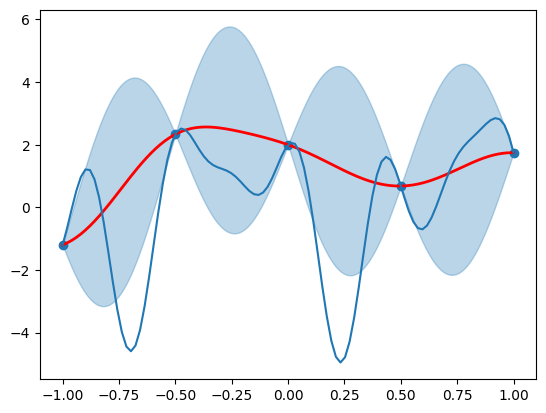
\includegraphics[width=0.3\linewidth]{images/iter_0.png}
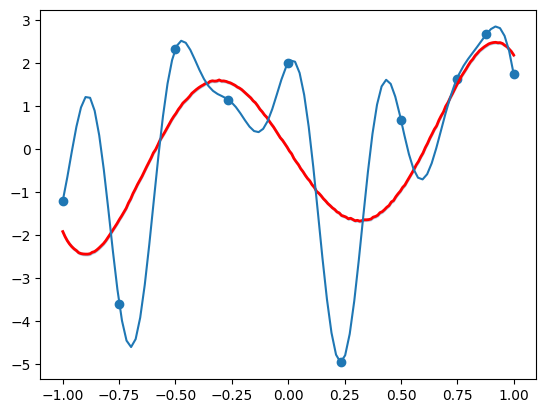
\includegraphics[width=0.3\linewidth]{images/iter_5.png}
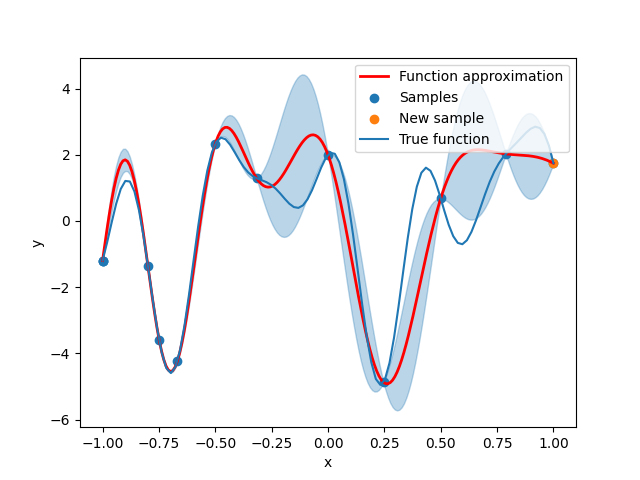
\includegraphics[width=0.3\linewidth]{images/iter_9.png}
\setlength{\belowcaptionskip}{-10pt}
\caption{Function approximation after adding each new data point according to our new rule, at iterations 0, 5 and 10 respectively.}
\label{fig:iter_new}
\end{figure}


%\begin{figure}[h]
%\centering
%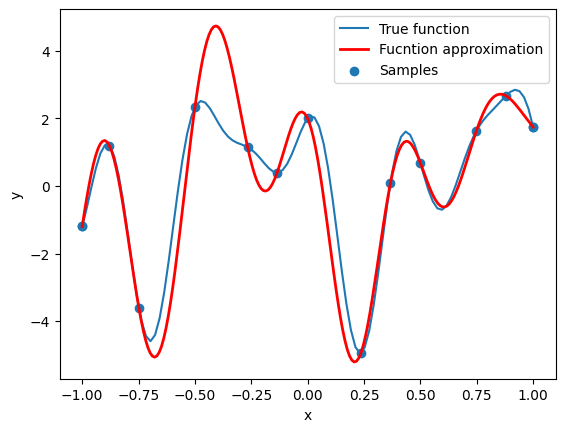
\includegraphics[width=0.5\linewidth]{images/output.png}
%\caption{GP Regression performed on the final dataset. The function now fits the original much better, and as a result gives a much better estimate of the minimum.}
%\label{fig:output}
%\end{figure}


\begin{figure}[h]
\centering
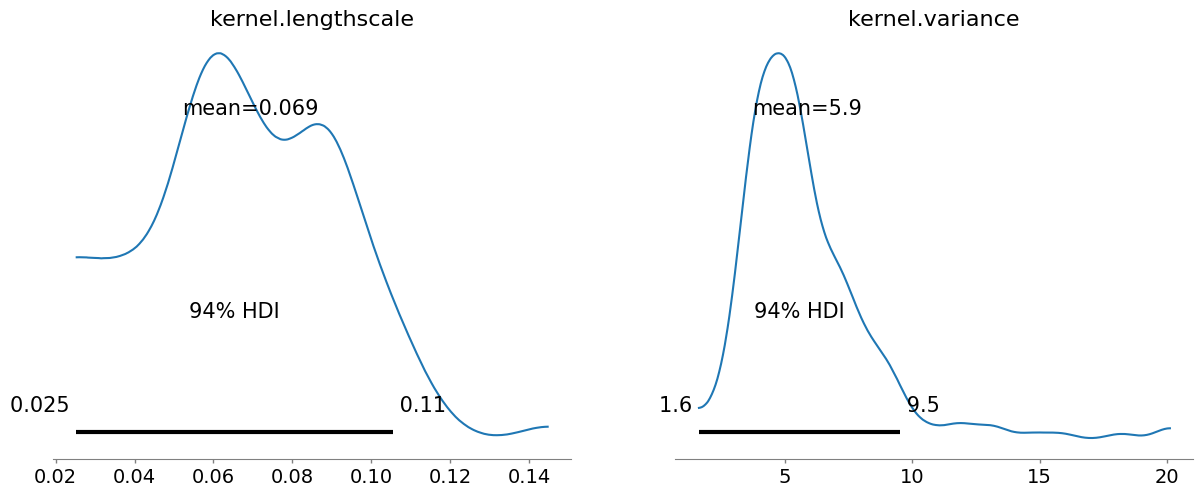
\includegraphics[width=0.49\linewidth]{images/arviz_0.png}
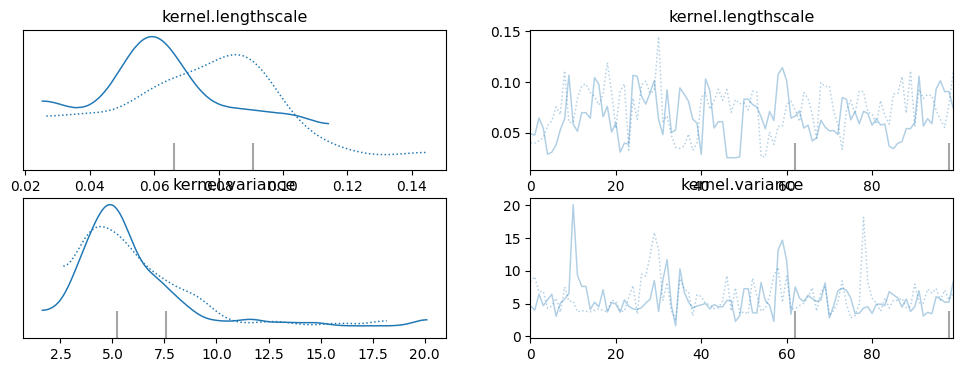
\includegraphics[width=0.49\linewidth]{images/arviz_1.png}
\setlength{\belowcaptionskip}{-10pt}
\caption{Arviz plots of the results using our formulation of the algorithm.}
\label{fig:arviz_new}
\end{figure}
